Il \textit{test driven development} (TDD) � una tecnica di programmazione che prevede la scrittura di un test, ovvero di una porzione di codice che si occupa di verificare una funzionalit�, prima della implementazione della funzionalit� stessa.

L'ideazione e la diffusione di questa tecnica di programmazione � stata curata da Kent Beck, che nel suo libro \textit{Test Driven Development: By Example} \cite{Beck:2002:TDD:579193} spiega come applicare il TDD a svariati contesti e dettaglia questa tecnica nelle sue tre fasi fondamentali, definite abitualmente con il termine \textit{red-green-refactor}. 

I nomi \textit{red} e \textit{green} delle prime due fasi derivano dalla convenzione, utilizzata dalla maggior parte dei framework di test, di indicare in colore rosso un test fallito e in verde un test andato a buon fine.

Di seguito sono riportati i dettagli di ciascuna fase.

\subsubsection{Prima fase: Red}
Ogni nuova feature da implementare inizia con la stesura di un nuovo test, questo aiuta il programmatore a definire, a priori, le specifiche funzionali della porzione di sistema che dovr� implementare. La funzionalit� descritta dal test pu� mappare direttamente una \textit{user story} o pu� essere una porzione di essa. 

Poich� la feature oggetto del test non � stata implementata, l'esecuzione del test riporter� esito negativo e, conseguentemente, esso risulter� fallito (rosso).

Questa pratica, a prima vista inutile, ha lo scopo di validare il test stesso. Infatti se il risultato fosse verde, questo significherebbe che esso � superfluo oppure errato.

\subsubsection{Seconda fase: Green}
Questa fase del processo � quella nella quale si esegue lo sviluppo vero e proprio della nuova funzionalit�, in modo da far diventare il test verde (soddisfatto). 

L'obbiettivo � esclusivamente soddisfare i requisiti quindi lo sviluppatore, tipicamente, cerca di arrivare alla soluzione nel modo pi� semplice possibile, non curandosi dei dettagli stilistici del codice.

\subsubsection{Terza fase: Refactor}
L'ultimo passo da eseguire � la rifattorizzazione del codice, cio� la riorganizzazione delle funzionalit� realizzate al passo precedente al fine di ottenere una architettura ben congegnata e una struttura chiara. 

Una delle tecniche principali per realizzare questo compito � chiamata \textit{Don't Repeat Yourself} (DRY) e consiste nel cercare di rimuovere quanto pi� possibile il codice duplicato mantenendo le medesime funzionalit�. 

L'utilizzo di questa tecnica favorisce il riuso e, tipicamente, veicola verso un buon design del software. In questa fase lo sviluppatore ha la massima libert� di sperimentazione, in quanto la correttezza del software rifattorizzato � garantita dai test scritti in precedenza. 

Il processo del TDD � iterativo, al termine della fase di refactoring, esso ricomincia da capo, con la stesura di un nuovo test o la riformulazione di test esistenti. Il grafico \ref{fig:red-green-refactor} riporta schematicamente l'andamento circolare di questo processo.

\begin{figure}[h]
\centering
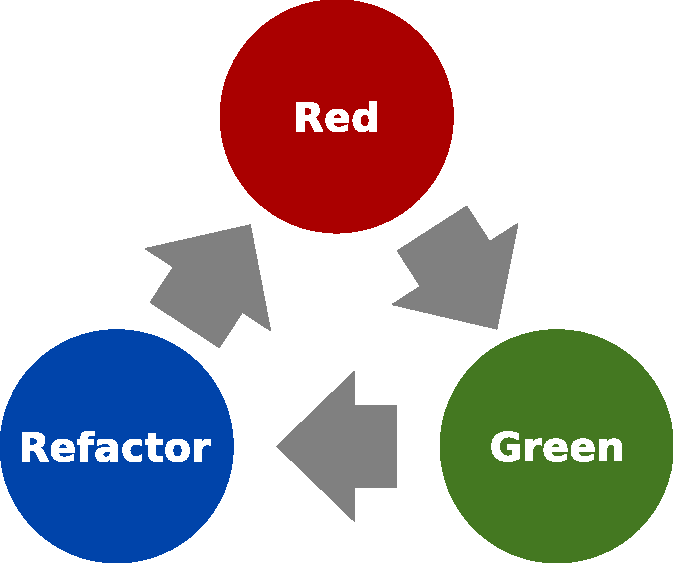
\includegraphics[width=0.7\linewidth]{./img/red-green-refactor}
\caption[Il flusso di lavoro circolare del TDD]{Il flusso di lavoro circolare del TDD}
\label{fig:red-green-refactor}
\end{figure}

La scelta di utilizzare il TDD all'interno di un progetto software garantisce la corretta implementazione delle user story. L'adozione di questa tecnica �, inoltre, facilitata dalla esistenza di innumerevoli framework di test per la maggior parte dei linguaggi di programmazione esistenti.

L'utilizzo del TDD fornisce agli sviluppatori svariati vantaggi, alcuni dei quali sono:
\begin{itemize}
\item riduzione drastica della necessit� di un \textit{debugger} per la ricerca degli errori;
\item acquisizione di fiducia nella sperimentazione, poich� l'impatto dell'adozione ogni soluzioni � sempre validato dai test e quantificabile;
\item documentazione del codice per gli altri sviluppatori del team, i test forniscono infatti esempi di utilizzo delle diverse funzionalit� implementate;
\item tracciamento dello stato di avanzamento dei lavori;
\item modularizzazione della struttura del progetto, tramite la suddivisione delle feature in unit� indipendenti e cooperanti tra loro;
\item \textit{focus} su una singola funzionalit�;
\end{itemize}